

\section{Methods}

\subsection{Downloading scripts used in this tutorial}

If one is interested to reproduce the workflow presented here, a good starting point would be to download the following GitHub repository:

\begin{verbatim}
git clone https://github.com/soda460/RNAseq_GATK_JGW.git
\end{verbatim}

It contains all scripts described in this section as well as several text files that allow to easily reproduce the analysis presented here. Note that some scripts use relative paths. Therefore using the files/folder organization presentend in figure 2 will help to reproduce the results presented here with minimal changes.



contained will also make the whole process easier.




\begin{figure}
\begin{center}

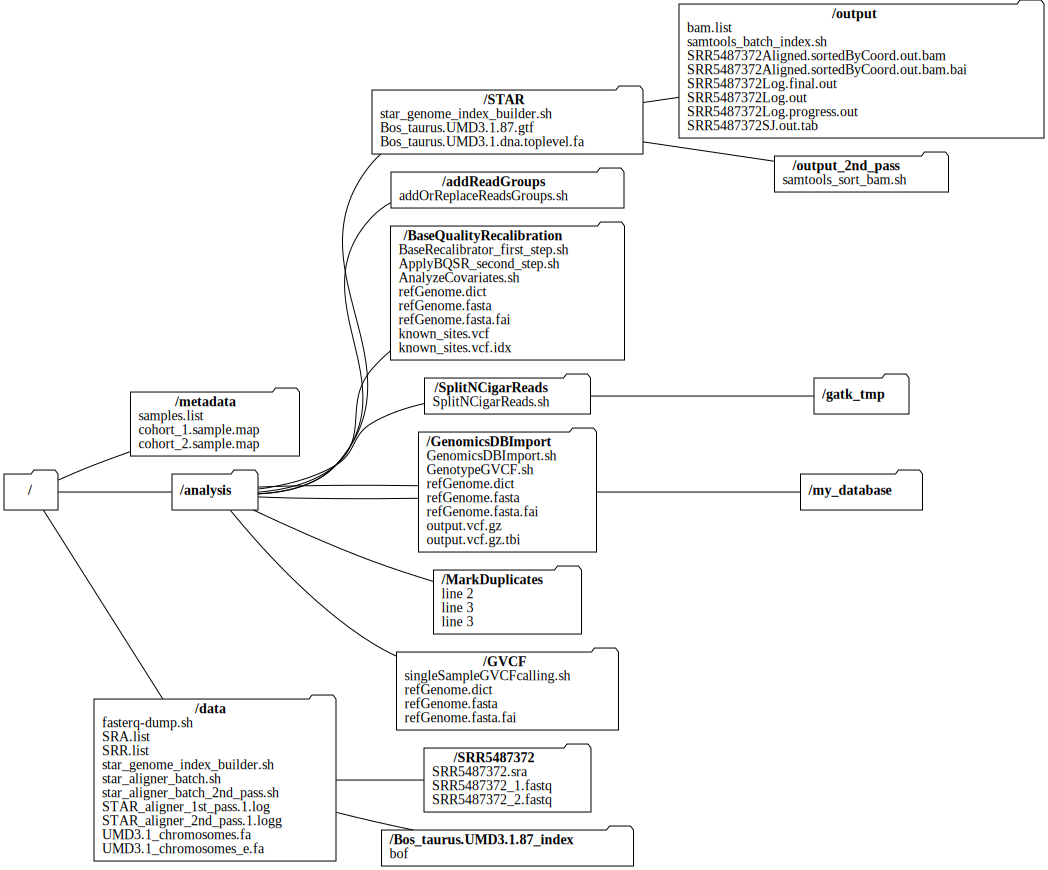
\includegraphics[width=1\textwidth]{misc/tree.png}
\caption[caption] {long desc.}

\end{center}
\end{figure}







\subsection{Downloading the MAP dataset from Sequence Read Archive}

We will use the complete RNA-seq raw sequences from \citep{Ariel2021}. However, rather than using the 72 samples presented in the article, we will focus on 24 representative samples of this study:

The \textbf{SRA.list} file contains the SRA identifiers of these 24 samples:
\begin{verbatim}
SRS2153774
SRS2153779
SRS2153781
SRS2153786
SRS2153787
SRS2153791
SRS2153793
SRS2153797
SRS2153799
SRS2153803
SRS2153805
SRS2153809
SRS2153811
SRS2153815
SRS2153817
SRS2153821
SRS2153823
SRS2153827
SRS2153829
SRS2153833
SRS2153835
SRS2153839
SRS2153841
SRS2153845
\end{verbatim}



Navigate to the /data directory and download the 24 samples with the the following command from the SRAtoolkit:

\begin{verbatim}
prefetch --option-file SRA.list
\end{verbatim}

To extract fastq files from .sra files, the fasterq-dump command is required. For example, the following command will produce SRR5487396\_R1.fastq.gz and SRR5487396\_R2.fastq.gz files from the SRR5487396.sra archive.

\begin{verbatim}
fasterq-dump --split-files SRR5487396/SRR5487396.sra
\end{verbatim}

In practice, you will want to extract all downloaded sequence read archives, which are nested in distinct folders. Navigate to the /data folder and use the following qsub command to lauch the faster-qdump commands sequentially:

\begin{verbatim}
qsub faster-qdump.sh
\end{verbatim}

where \textbf{faster-qdump.sh} is a bash script containing instructions for the SGE workload manager and the code to iterate on all downloaded sequence read archives and produce the forward and reverse fastq files:

\begin{verbatim}
#! /bin/bash
#$ -S /bin/bash
#$ -cwd
#$ -N 'fasterq-dump'
#$ -pe smp 12
#$ -o ./qsub_log.txt
#$ -e ./qsub_err.txt
	
for i in `ls -d SRR*`; do
	cd $i
	fasterq-dump --split-files $i.sra
	cd ..
done
\end{verbatim}



However, execute the latter script would take a lot of times. To take advantage of the capacity of the cluster, one should may consider launching array tasks (task in parallel). To learn more about this, one can visit this page (SGE).

Before using the faster-qdump\_parallel.sh, we need to create a simple list file of the 24 SRR* folders present in the /data folder:

\begin{verbatim}
ls -d1 SRR5487???>SRR.list
\end{verbatim}

Be sure that the SRR.list file contains the 24 SRR identifiers (without the .sra extension) on separates lines before lauching the paralle version of fasterq.dump.sh which look like:

\begin{verbatim}
#!/bin/bash
#$ -V
#$ -N fasterq-dump
#$ -S /bin/bash
#$ -cwd
#$ -j y
#$ -b n
#$ -e ./qsub_err.txt
#$ -o ./qsub_log.txt
#$ -q all.q
#$ -t 1-24
#$ -pe smp 4

input=$(head -n $SGE_TASK_ID SRR.list | tail -n 1)

fasterq-dump --split-files $input/$input.sra
\end{verbatim}


Figure x show how a computationnaly intense task, namely the decompressing of an .sra archive, can be run at the same time with different input files. This can be done by using the SGE task array capabilities. Technically, the same script is run multiple times, with different values taken by the single environment variable \$SGE\_TASK\_ID. Since many bioinformatic tasks used in this tutorial are computationally intensive, most of the scripts presented thereafter will be base on this model.




%figure file organization



 

\subsection{Performing STAR alignment}

\subsubsection{Generating genome indexes files}

STAR genomes are available for a limited number of genomes on the gingeras lab. We will use the for \textit{Bos taurus}  UMD3.1.87 annotations file since the BosTau7 version of the genome was used in \cite{Ariel2021}. The GTF file describe all exons whereas the .dna.toplevel.fa fasta file contains the corresponding sequences.



\begin{verbatim}
wget http://labshare.cshl.edu/shares/gingeraslab/www-data/dobin/\
STAR/STARgenomes/Old/ENSEMBL/bos_taurus/Bos_taurus.UMD3.1.87.gtf;

wget http://labshare.cshl.edu/shares/gingeraslab/www-data/dobin/\
STAR/STARgenomes/Old/ENSEMBL/bos_taurus/Bos_taurus.UMD3.1.dna.toplevel.fa;
\end{verbatim}

To prepare genome index files for STAR, use the genomeGenerate built-in STAR command.
Note that you have to create a directory where STAR could buid the index.

\begin{verbatim}
mkdir Bos_taurus.UMD3.1.87_index
\end{verbatim}

 as in the following script:

\begin{verbatim}
cat Bos_taurus.UMD3.1.87_index/chrName.txt | head -n 34
\end{verbatim}

\textbf{star\_genome\_index\_builder.sh}
\begin{verbatim}
#! /bin/bash
#$ -S /bin/bash
#$ -cwd
#$ -N 'STAR_genome_builder'
#$ -pe smp 6
#$ -o ./qsub_log.txt
#$ -e ./qsub_err.txt
STAR --runThreadN 6 \
--runMode genomeGenerate \
--genomeDir Bos_taurus.UMD3.1.87_index \
--genomeFastaFiles ./Bos_taurus.UMD3.1.dna.toplevel.fa \
--sjdbGTFfile ./Bos_taurus.UMD3.1.87.gtf \
--sjdbOverhang 99
\end{verbatim}






\subsubsection{Aligment with the STAR aligner}

At this step, we align our raw .fastq files with the STAR aligner.

%STAR fisrt pass
\begin{verbatim}
#!/bin/bash
#$ -V
#$ -N 'STAR_aligner'
#$ -S /bin/bash
#$ -cwd
#$ -j y
#$ -b n
#$ -e e
#$ -o STAR_aligner_1st_pass.$TASK_ID.log
#$ -q all.q
#$ -t 1-24
#$ -pe smp 4


input=$(head -n $SGE_TASK_ID SRR.list | tail -n 1)


mkdir -p ../analysis/STAR/output/$input

STAR --genomeDir ./Bos_taurus.UMD3.1.87_index \
--runThreadN 12 \
--readFilesIn  ./$input/$input"_1.fastq" ./$input/$input"_2.fastq" \
--outFileNamePrefix ../analysis/STAR/output/$input \
--outSAMtype BAM SortedByCoordinate \
--outSAMunmapped Within \
--outSAMattributes Standard
\end{verbatim}



\subsubsection{Adding Splice junctions (2nd mapping pass)}

GATK workflow recommend to perform 2-pass mapping with the STAR aligner. The 2nd mapping pass is identical to the first alignment except that all splice junctions discovered in the first pass are given as input to the programs, allowing to XXXX. Simply specify a list of all splice junctions files after the --sjdbFileChrStartEnd argument.


\begin{verbatim}
----outTmpDir ../analysis/STAR/output_2nd_pass/_STARtmp_$TASK_ID \
\end{verbatim}

%STAR 2nd pass listing
\begin{verbatim}
#!/bin/bash
#$ -V
#$ -N 'STAR_aligner_2nd_pass'
#$ -S /bin/bash
#$ -cwd
#$ -j y
#$ -b n
#$ -e e
#$ -o STAR_aligner_2nd_pass.$TASK_ID.log
#$ -q all.q
#$ -t 1-24
#$ -pe smp 4


input=$(head -n $SGE_TASK_ID SRR.list | tail -n 1)

mkdir -p ../analysis/STAR/output_2nd_pass/$input

STAR --genomeDir ./Bos_taurus.UMD3.1.87_index \
--runThreadN 4 \
--readFilesIn  ./$input/$input"_1.fastq" ./$input/$input"_2.fastq" \
--outFileNamePrefix ../analysis/STAR/output_2nd_pass/$input \
--outSAMtype BAM SortedByCoordinate \
--outSAMunmapped Within \
--outSAMattributes Standard \
--outTmpDir ../analysis/STAR/output_2nd_pass/_STARtmp_$SGE_TASK_ID \
--sjdbFileChrStartEnd \
../analysis/STAR/output/SRR5487372SJ.out.tab \
../analysis/STAR/output/SRR5487384SJ.out.tab \
../analysis/STAR/output/SRR5487396SJ.out.tab \
../analysis/STAR/output/SRR5487408SJ.out.tab \
../analysis/STAR/output/SRR5487420SJ.out.tab \
../analysis/STAR/output/SRR5487432SJ.out.tab \
../analysis/STAR/output/SRR5487376SJ.out.tab \
../analysis/STAR/output/SRR5487388SJ.out.tab \
../analysis/STAR/output/SRR5487400SJ.out.tab \
../analysis/STAR/output/SRR5487412SJ.out.tab \
../analysis/STAR/output/SRR5487424SJ.out.tab \
../analysis/STAR/output/SRR5487436SJ.out.tab \
../analysis/STAR/output/SRR5487378SJ.out.tab \
../analysis/STAR/output/SRR5487390SJ.out.tab \
../analysis/STAR/output/SRR5487402SJ.out.tab \
../analysis/STAR/output/SRR5487414SJ.out.tab \
../analysis/STAR/output/SRR5487426SJ.out.tab \
../analysis/STAR/output/SRR5487438SJ.out.tab \
../analysis/STAR/output/SRR5487382SJ.out.tab \
../analysis/STAR/output/SRR5487394SJ.out.tab \
../analysis/STAR/output/SRR5487406SJ.out.tab \
../analysis/STAR/output/SRR5487418SJ.out.tab \
../analysis/STAR/output/SRR5487430SJ.out.tab \
../analysis/STAR/output/SRR5487442SJ.out.tab

\end{verbatim}



\subsubsection{Sorting alignment files}


After you align your sequences. You will want that your .bam files to be indexed and sorted by coordinates. As mentioned earlier, STAR allows the output to be sorted by coordinates. If you have carefully followed this tutorial, there is no need to sort again your bam files and you can safely ignore the next step and jump to the next subheading. However, if for any reasons, your aligmnents files are not sorted adequately, the sort option of samtools is as easy as :

\begin{verbatim}
samtools sort file.bam -o file_sorted.bam
\end{verbatim}

In a folder containing unsorted alignment, first prepare a list of bam files to be sorted with:

\begin{verbatim}
ls -1 *.bam > bam.list
\end{verbatim}

For our data, a qsub script would allow to re-sort our alignments files:


% samtools sort listing
\begin{verbatim}
#!/bin/bash
#$ -V
#$ -N samtools_sort
#$ -S /bin/bash
#$ -cwd
#$ -j y
#$ -b n
#$ -e e
#$ -o o
#$ -q all.q
#$ -t 1-24
#$ -pe smp 2

input=$(head -n $SGE_TASK_ID bam.list | tail -n 1 | xargs basename -s '.bam')

samtools sort $input.bam -o $input"_sorted.bam"

\end{verbatim}

Note that this listing could be used as a template to perform a variety of samtools subcommands that involve renaming the output files.


\subsubsection{Indexing alignment files}

BAM files (the binary analog of Sequence Alignment Mapping (SAM) files) are very efficient bioinformatic files designed to store high-throughput alignment data. Typically, they contain the result of the alignment of millions of sequencing reads against a reference genome and greatly benefit from being  indexed by genomic positions for faster random access to the aligned reads at a specific locus. In practice most programs will complain if in the absence of index files. Note that BAM files need to be sorted before being indexed. To index all bam files present in the STAR output\_2nd\_pass folder, first prepare a list of bam files to be indexed with:

\begin{verbatim}
ls -1 *.bam > bam.list
\end{verbatim}

then, you can index all alignements in parallel with:

\begin{verbatim}
qsub samtools_batch_index.sh
\end{verbatim}

where the latter script looks like:

%samtools index listing
\begin{verbatim}
#!/bin/bash
#$ -V
#$ -N samtools_index
#$ -S /bin/bash
#$ -cwd
#$ -j y
#$ -b n
#$ -e e
#$ -o o
#$ -q all.q
#$ -t 1-24
#$ -pe smp 2

input=$(head -n $SGE_TASK_ID bam.list | tail -n 1)

samtools index $input
\end{verbatim}





\subsection{Adding Read groups}

Contrarily to fastq, SAM files have the capacity to handle large amount of metadata. A good practice would be to include informations about the reference genome and the samples in aligment files. Informations about the processing steps could also be stored in alignment files. Many programs, such as GATK, will add this metadata information when manipulating SAM/BAM files.


Before running any GATK workflow, one will need to add Read groups. This step ensure that relevant informations about the sequencing process are assigned to each read in an alignment file. When this step is done carefully, it allow to mitigate the consequences of the sequencing biais that might arise due to how the sequencing process was performed \cite{GATK_ReadGroups}. For example, when samples are multiplexed, it is important to known which reads origin from the same library, which were sequenced on the same flowcell, etc. The GATK engine requires the presence of several read group fields to run without errors. To learn more about the Read groups as understant by the GATK team and to learn how to derive this information from read names, one should consult this page: \href{https://gatk.broadinstitute.org/hc/en-us/articles/360035890671-Read-groups}{https://gatk.broadinstitute.org/hc/en-us/articles/360035890671-Read-groups}.

Here, we will set the flowcells, sequencing lanes and sample barcode in the PU (Platform Unit) tag. We will also set the PL (Platform/technology used to produce the read) and LB (DNA preparation library identifier) tags. Note that we do not need to set any ID (Read group identifier) is overrided by the PU tag for base recalibration when it is defined.


Before running the main script, we will extract the first and fifth columns from our metadata file and place them in separate files, namely RGLB.txt and  RGPU.txt, that will be further used to populate the LB and PU read groups fields:

\begin{verbatim}
# Corresponding to the sample name
cut -f 1 -d ',' ../../metadata/metadata.txt | tail -n +2 > RGLB.txt

# Corresponding to the PU tag FLOW CELL 
cut -f 5 -d ',' ../../metadata/metadata.txt | tail -n +2 > RGPU.txt
\end{verbatim}

where /metadata/metadata.txt looks like:

\begin{verbatim}
sample,cowID,SRAID,Run,RGPU
A_CTL24,cowA,SRS2153774,SRR5487372,C5NL3ACXX.1.CAGATC
A_MAP24,cowA,SRS2153779,SRR5487376,C5NL3ACXX.1.TGACCA
B_CTL24,cowB,SRS2153781,SRR5487378,C5NL3ACXX.3.TGACCA
B_MAP24,cowB,SRS2153786,SRR5487382,C5NL3ACXX.3.GTGAAA
C_CTL24,cowC,SRS2153787,SRR5487384,C5K8FACXX.3.AGTCAA
C_MAP24,cowC,SRS2153791,SRR5487388,C5K8FACXX.3.GTCCGC
D_CTL24,cowD,SRS2153793,SRR5487390,C5K8FACXX.1.TGACCA
D_MAP24,cowD,SRS2153797,SRR5487394,C5K8FACXX.1.GTGAAA
E_CTL24,cowE,SRS2153799,SRR5487396,C547FACXX.1.AGTCAA
E_MAP24,cowE,SRS2153803,SRR5487400,C547FACXX.1.GTCCGC
F_CTL24,cowF,SRS2153805,SRR5487402,C547FACXX.3.TGACCA
F_MAP24,cowF,SRS2153809,SRR5487406,C547FACXX.3.GTGAAA
G_CTL24,cowG,SRS2153811,SRR5487408,C5NL3ACXX.5.AGTCAA
G_MAP24,cowG,SRS2153815,SRR5487412,C5NL3ACXX.5.GTCCGC
H_CTL24,cowH,SRS2153817,SRR5487414,C5NL3ACXX.7.TGACCA
H_MAP24,cowH,SRS2153821,SRR5487418,C5NL3ACXX.7.CTTGTA
I_CTL24,cowI,SRS2153823,SRR5487420,C5K8FACXX.5.AGTTCC
I_MAP24,cowI,SRS2153827,SRR5487424,C5K8FACXX.5.GTGAAA
J_CTL24,cowJ,SRS2153829,SRR5487426,C5K8FACXX.7.TGACCA
J_MAP24,cowJ,SRS2153833,SRR5487430,C5K8FACXX.7.GTGAAA
K_CTL24,cowK,SRS2153835,SRR5487432,C547FACXX.5.AGTCAA
K_MAP24,cowK,SRS2153839,SRR5487436,C547FACXX.5.GTCCGC
L_CTL24,cowL,SRS2153841,SRR5487438,C547FACXX.7.AGTCAA
L_MAP24,cowL,SRS2153845,SRR5487442,C547FACXX.7.GTCCGC
\end{verbatim}


The RGLB.txt file will therefore hold the library name for each 24 samples (e.g. C\_MAP24, which design a RNAseq library done on the cow C 24h post-infection with the MAP pathogen). The RGPU.txt hold the Platform Unit tag, which is made of three types of informations: the flowcell, sequencing lane and barcode identifiers, with the following format: {FLOWCELL\_BARCODE}.{LANE}.{SAMPLE\_BARCODE}. 


We use the following script to add read groups in our alignments files. Note that bash arrays are zero-indexed. It is why, we use the value given by \$SGE\_TASK\_ID -1 (0-23) to fetch the correct values in RGLB and RGPU arrays.

%AddOrReplaceReadGroups listing
\begin{verbatim}
#!/bin/bash

#$ -V
#$ -N AddOrReplaceReadGroups
#$ -S /bin/bash
#$ -cwd
#$ -j y
#$ -b n
#$ -e e
#$ -o logfile.txt
#$ -q all.q
#$ -t 1-24
#$ -pe smp 1

eval "$(conda shell.bash hook)"
conda activate gatk4

SAMPLES="$HOME/jsb/springer2/RNAseq_GATK_JGW/metadata/samples.list"
BAMPATH="$HOME/jsb/springer2/RNAseq_GATK_JGW/analysis/STAR/output_2nd_pass"
OUTPUT="$HOME/jsb/springer2/RNAseq_GATK_JGW/analysis/addReadGroups"

readarray -t RGLB < ./RGLB.txt
readarray -t RGPU < ./RGPU.txt

input=$(head -n $SGE_TASK_ID $SAMPLES | tail -n 1)

java -jar $PICARD AddOrReplaceReadGroups \
I=$BAMPATH/$input"Aligned.sortedByCoord.out.bam" \
O=$OUTPUT/$input".bam" \
RGLB=${RGLB[$SGE_TASK_ID -1]} \
RGPL=ILLUMINA \
RGPU=${RGPU[$SGE_TASK_ID -1]} \
RGID=${RGPU[$SGE_TASK_ID -1]} \
RGSM=$input

conda deactivate
\end{verbatim}


It is highly recommended to validate such editing tasks. Using a simple UNIX trick alloes one to see the read groups of a .bam files:

\begin{verbatim}
samtools view -H $i.bam | grep '@RG'	
\end{verbatim}

With our data, we can iterate on all .bam files and ensure that the reads groups have been correctly set:

\begin{verbatim}
for i in `tail -n +2 ../../metadata/metadata.txt | cut -f 4 -d ','`; do echo $i; samtools view -H $i.bam | grep '@RG'; done
\end{verbatim}






\subsection{MarkDuplicates}


Duplicate reads can arise from PCR duplication artifacts that take place during the library construction or from reading errors that occur during the sequencing process (optical duplicates). Regardless of their origin, these reads need to be identified in alignment files. The MarkDuplicate program from the Picard tools have many options to deal with these issue and output some metrics. For example, the program offer the possibility to completely remove the duplicate reads and to make the distinction between optical and PCR duplicates.

Here we will simply identified the duplicate reads in our .bam files before proceeding to the next step:

%MarkDuplicate script
\begin{verbatim}
#!/bin/bash
#$ -V
#$ -N samtools_index
#$ -S /bin/bash
#$ -cwd
#$ -j y
#$ -b n
#$ -o logfile.$TASK_ID.log
#$ -q all.q
#$ -t 1-24
#$ -pe smp 2

SAMPLES="$HOME/jsb/springer/metadata/samples.list"
BAMPATH="$HOME/jsb/springer/analysis/addReadGroups"
OUTPUT="$HOME/jsb/springer/analysis/MarkDuplicates"

input=$(head -n $SGE_TASK_ID $SAMPLES | tail -n 1)

java -jar $PICARD MarkDuplicates \
I=$BAMPATH/$input".bam" \
O=$OUTPUT/$input"_marked_duplicates.bam" \
M=$OUTPUT/$input"_marked_dup_metrics.txt"
\end{verbatim}

\subsection{SplitNCigarReads}

Along with the non-GATK alignment of RNAseq raw sequences, the SplitNCigarReads step, called SplitNTrim in the previous versions of GATK workflows, is highly specific to RNAseq analysis. During this step reads that span splice junctions (for example reads that align over distinct exons) are split in smaller reads during the process. This step will produce alignments files that will adequately represent reads that span splice junctions. However, before doing this step, we need to get and prepare reference genome files.

(Distinguish between hard and soft clipped).


\subsubsection{Preparing reference genome files}

Until now, we have work with STAR reference genome which barely contains sequences that are transcribed in RNA. In contrast, the GATK SplitNCigarReads command requires to use a complete reference sequence. At this point, one should be advised to download the same version of the full refence genome that was used to prepare the STAR genome.

To get the UMD3.1 assembly, visit \href{https://bovinegenome.elsiklab.missouri.edu/}{https://bovinegenome.elsiklab.missouri.edu/} and download the UMD3.1\_chromosomes.fa.gz and Ensembl79\_UMD3.1\_genes.gff3.gz files.


It is crucial that entries in the reference genome match the corresponding ones in the STAR genome. If you inspect the fasta headers of the UMD3.1\_chromosomes.fa, you will notice that each fasta entry contains many fields (e.g. gnl , UMD3.1 Accession numbers):

\begin{verbatim}
grep ">" UMD3.1_chromosomes.fa
\end{verbatim}


\begin{verbatim}
>gnl|UMD3.1|GK000010.2 Chromosome 10 AC_000167.1
>gnl|UMD3.1|GK000011.2 Chromosome 11 AC_000168.1
>gnl|UMD3.1|GK000012.2 Chromosome 12 AC_000169.1
...
>gnl|UMD3.1|GJ060407.1 GPS_000344847.1 NW_003101152.1
>gnl|UMD3.1|GJ060408.1 GPS_000344848.1 NW_003101153.1
\end{verbatim}

In contrast, the chromosomes entries in the STAR genome are quite different:

\begin{verbatim}
cat XXXX file in STAR genome
\end{verbatim}



One could use the following commands to rename the chromosome identifiers found in the Bos taurus UMD3.1 genome to the plain chromosome numbers as what is seen in the STAR genome:

\begin{verbatim}
sed -r s'/^>.+Chromosome\s+(\S+)\s+.+/>\1/' UMD3.1_chromosomes.fa > temp1.fa
grep ">" temp1.fa | head -n 40
sed -r s'/^>gnl\|UMD3\.1\|(\S+)+\s+.+/>\1/' temp1.fa > temp2.fa
grep ">" temp2.fa | tail -n +30 | head -n 10
mv temp2.fa refGenome.fasta
rm temp1.fa
\end{verbatim}


Along with the reference genome, many GATK tools will need a dictionary file ending in .dict and an index file ending in .fai.\href{ https://gatk.broadinstitute.org/hc/en-us/articles/360035531652-FASTA-Reference-genome-format}{ https://gatk.broadinstitute.org/hc/en-us/articles/360035531652-FASTA-Reference-genome-format}). These files need to share the same basename as the reference genome. You can prepare the index with:

\begin{verbatim}
samtools faidx refGenome.fasta
\end{verbatim}

On the other hand, use the GATK CreateSequenceDictionary tool to create the required .dict file:

\begin{verbatim}
gatk CreateSequenceDictionary -R refGenome.fasta
\end{verbatim}




\subsubsection{Running SplitNCigarReads}

Having prepared reference genome files and index, we are ready to lauch the following SplitNCigarRead listing:

\begin{verbatim}
#!/bin/bash
#$ -V
#$ -N SplitNCigarReads
#$ -S /bin/bash
#$ -cwd
#$ -j y
#$ -b n
#$ -e e
#$ -o SplitNCigarReads.$TASK_ID.log
#$ -q all.q
#$ -t 1-24
#$ -pe smp 4
	
eval "$(conda shell.bash hook)"
conda activate gatk4
	
SAMPLES="$HOME/jsb/springer/metadata/samples.list"
BAMPATH="$HOME/jsb/springer/analysis/MarkDuplicates"
OUTPUT="$HOME/jsb/springer/analysis/SplitNCigarReads"
	
input=$(head -n $SGE_TASK_ID $SAMPLES | tail -n 1)

gatk SplitNCigarReads \
-R refGenome.fasta \
-I $BAMPATH/$input"_marked_duplicates.bam" \
-O $OUTPUT/$input"_SplitNCigarReads.bam" \
--tmp-dir $output/gatk_tmp
	
conda deactivate
\end{verbatim}



\subsection{Performing base quality score recalibration}

Base Quality Score Recalibration (BQSR) is an optional, but highly recommended step, that figure in DNAseq and RNAseq GATK best practices workflows. This complex procedure, which involves binning and machine learning consist of re-evaluating all base quality scores assigned by sequencing machines which are prone to systematic technical errors \cite{GATK_BaseQuality}. This procedure lead to more accurate base calls, a situation that improve the accuracy of variant calling overall. More details about how the model is build and how new quality scores are computed can be found at \href{https://gatk.broadinstitute.org/hc/en-us/articles/360035890531-Base-Quality-Score-Recalibration-BQSR-}{https://gatk.broadinstitute.org/hc/en-us/articles/360035890531-Base-Quality-Score-Recalibration-BQSR-}.

\subsubsection{Using BaseRecalibrator}

In the first key step  a model of covariation is build with two components: the alignement given as input (bam files) and a set of known variants (VCF file). The BaseRecalibrator will then produce a recalibration file which is used in the second key step of the procedure. To perform this task one would need a source of reliable variants in the investigated genome. With human data and other common model organisms, it would be easy to find such sources of variants thanks to the existence of variation databases. Here we use a single VCF file containing the results of SNP50 beadchip genotyping to train the model, but you can feed the model with many VCF files.

%BaseRecalibrator first script
\begin{verbatim}
#!/bin/bash
#$ -V
#$ -N BaseRecalibrator
#$ -S /bin/bash
#$ -cwd
#$ -j y
#$ -b n
#$ -e e
#$ -o BaseQualityRecalibration_$TASK_ID.log
#$ -q all.q
#$ -t 1-24
#$ -pe smp 4

eval "$(conda shell.bash hook)"
conda activate gatk4

SAMPLES="$HOME/jsb/springer/metadata/samples.list"
BAMPATH="$HOME/jsb/springer/analysis/SplitNCigarReads"
OUTPUT="$HOME/jsb/springer/analysis/BaseQualityRecalibration"

input=$(head -n $SGE_TASK_ID $SAMPLES | tail -n 1)

gatk BaseRecalibrator \
-R ./refGenome.fasta \
-I $BAMPATH/$input"_SplitNCigarReads.bam" \
--known-sites ./jsb.vcf \
-O $OUTPUT/$input"_recal_data.table"

conda deactivate
\end{verbatim}





\subsubsection{Using ApplyBQSR to adjust the scores}

In the second step of the BaseQuality recalibration process, the GATK ApplyBQSR command assigns new scores to each base based on the model produced in the first step and produces new BAM files that reflet these changes.  


%ApplyBQSR listing
\begin{verbatim}
#!/bin/bash

#$ -V
#$ -N ApplyBQSR
#$ -S /bin/bash
#$ -cwd
#$ -j y
#$ -b n
#$ -e e
#$ -o ApplyBQSR_$TASK_ID.log
#$ -q all.q
#$ -t 1-24
#$ -pe smp 4

eval "$(conda shell.bash hook)"
conda activate gatk4

SAMPLES="$HOME/jsb/springer/metadata/samples.list"
BAMPATH="$HOME/jsb/springer/analysis/SplitNCigarReads"
OUTPUT="$HOME/jsb/springer/analysis/BaseQualityRecalibration"

echo $SAMPLES
input=$(head -n $SGE_TASK_ID $SAMPLES | tail -n 1)

gatk ApplyBQSR \
-R ./refGenome.fasta \
-I $BAMPATH/$input"_SplitNCigarReads.bam" \
--bqsr-recal-file $OUTPUT/$input"_recal_data.table" \
-O $OUTPUT/$input"_recal.bam"

conda deactivate
\end{verbatim}

\subsubsection{Comparing pre- and post-recalibration metrics}

To visualize the effect of the procedure, one can build a seconde model and generate plots with data before and after recalibration \cite{GATK_BaseQuality} The GATK command AnalyzeCovariates was created for that purpose as in the following example:

\begin{verbatim}
gatk AnalyzeCovariates \
-before recal1.table \
-after recal2.table \
-plots AnalyzeCovariates.pdf
\end{verbatim}



\subsection{Joint genotyping Variant Calling}


Best practices workflow 


More details about the incremental discovery can be found here:

\subsubsection{Variant calling (ERC mode)}
%GCVF listing


In this step, the GATK variant calling engine, HaplotypeCaller, identifies potential variation sites and record them in GVCF files. This is why this step has been called "GVCF workflow". GVCF files act as intermediate between analysis ready reads (BAM files) and the final joint analysis of multiple samples \cite{GATK_jointCalling_1}. Such intermediate files facilitate the incremental discovery of variants and should be kept since they can be reused in novel rounds of joint genotyping analysis. Our listing to produce GVCF files for each sample reads as follow:


\begin{verbatim}
#!/bin/bash
#$ -V
#$ -N callingGVCF
#$ -S /bin/bash
#$ -cwd
#$ -j y
#$ -b n
#$ -e e
#$ -o singleSampleCallingGVCF_$TASK_ID.log
#$ -q all.q
#$ -t 1-24
#$ -pe smp 4

eval "$(conda shell.bash hook)"
conda activate gatk4

SAMPLES="$HOME/jsb/springer/metadata/samples.list"
BAMPATH="$HOME/jsb/springer/analysis/BaseQualityRecalibration"
OUTPUT="$HOME/jsb/springer/analysis/GVCF"

echo $SAMPLES
input=$(head -n $SGE_TASK_ID $SAMPLES | tail -n 1)

gatk --java-options "-Xmx4g" HaplotypeCaller \
-R ./refGenome.fasta \
-I $BAMPATH/$input"_recal.bam" \
-O $OUTPUT/$input".g.vcf.gz" \
-ERC GVCF

conda deactivate
\end{verbatim}





\subsubsection{Merge of GCVF files}

This step has been revised recently by GATK experts by the addition of the novel GATK GenomicsDBImport command. It resembles the former CombineGVCFs command, but promises better performances for parsing of VCF files and computing of values stored in the VCF INFO fields. More details can be found at \href{https://gatk.broadinstitute.org/hc/en-us/articles/360036883491-GenomicsDBImport}{https://gatk.broadinstitute.org/hc/en-us/articles/360036883491-GenomicsDBImport}. The command requires a map files that list the full paths of all GVCF files to be included in the resulting database. 

The -L option specifies the range genomic intervals on which the command operate and may be used several times. Since, we are interested to call variants on all bovine autosomes, we used it many times in the following listing:


%GenomicsDBImport listing
\begin{verbatim}
eval "$(conda shell.bash hook)"
conda activate gatk4

SAMPLES="$HOME/jsb/springer/metadata"
OUTPUT="$HOME/jsb/springer/analysis/GenomicsDBImport"

gatk --java-options "-Xmx4g -Xms4g" \
GenomicsDBImport \
--genomicsdb-workspace-path $OUTPUT/"my_database" \
-L 1 \
-L 2 \
-L 3 \
-L 4 \
-L 5 \
-L 6 \
-L 7 \
-L 8 \
-L 9 \
-L 10 \
-L 11 \
-L 12 \
-L 13 \
-L 14 \
-L 15 \
-L 16 \
-L 17 \
-L 18 \
-L 19 \
-L 20 \
-L 21 \
-L 22 \
-L 23 \
-L 24 \
-L 25 \
-L 26 \
-L 27 \
-L 28 \
-L 29 \
--sample-name-map $SAMPLES/"cohort_1.sample_map" \
--tmp-dir $HOME/jsb/tmp \
--reader-threads 5
conda deactivate

\end{verbatim}


\subsubsection{Joint genotyping}

The final step in this variant calling workflow, which is actually the joint genotyping step, is performed with the GATK GenotypeGVCFs command at  \href{https://gatk.broadinstitute.org/hc/en-us/articles/360037057852-GenotypeGVCFs}{https://gatk.broadinstitute.org/hc/en-us/articles/360037057852-GenotypeGVCFs}. During this operation, all samples for which variant have been pre-called with HaplotypeCaller are jointly genotyped. The command take as argument a GenomicsDB workspace created by GenomicsDBImport, which is barely a database of GVCF files produced by the HaplotypeCaller. Alternatively, a single multi-sample GCVF file produced by CombineGVCFs (used after HaplotypeCaller) can also be given as input.

%GenotypeGVCFs listing
\begin{verbatim}
#!/bin/bash
#$ -V
#$ -N GenotypeGVCF
#$ -S /bin/bash
#$ -cwd
#$ -j y
#$ -b n
#$ -e e
#$ -o GenotypeGVCF.log
#$ -q all.q
#$ -pe smp 4

eval "$(conda shell.bash hook)"
conda activate gatk4

gatk --java-options "-Xmx4g" GenotypeGVCFs \
-R refGenome.fasta \
-V gendb://my_database \
-O output.vcf.gz
conda deactivate
\end{verbatim}






\subsection{Examine and visualize alignment files}

At this step, you could examine your alignments files.

Tablet (https://ics.hutton.ac.uk/tablet/download-tablet/) is a good program to visualize alignments files. The IVG viewer could also be used.


One should always keep a copy of the VCF output file in a safe place. It is fairly common to corrput a .gz file with compressing/decompressing operations.




\begin{verbatim}
gunzip -c output.vcf.gz > output.vcf
\end{verbatim}





\subsubsection{The gff3 file}

With the command below, one can see the number of features annotated for each ID in the gff3 file: 

\begin{verbatim}{bash}
cat Ensembl79_UMD3.1_genes.gff3 | cut -f 1 | uniq -cd
\end{verbatim}


%output of cat Ensembl79 gff3
Here a summary of the previous command:
\begin{verbatim}
21287 GK000001.2
18819 GK000030.2
26235 GK000002.2
29793 GK000003.2
...
14 GJ058430.1
31 GJ058425.1
...
23 GJ059509.1
3 GJ058729.1
3 GJ060027.1
3 GJ058256.1
\end{verbatim}

Therefore, to ensure that the gff3 chromosome IDs match those presennt in our alignment files, we need to slightly edit this file to replace the pattern used for the chromosome IDs (GK + 0000 + chromosome number) by solely the chromosome number. This could be done easily with sed:

\begin{verbatim}
sed -r s'/^GK[0]+([0-9]+).2/\1/'g Ensembl79_UMD3.1_genes.gff3 \
> Ensembl79_UMD3.1_genes_e.gff3
\end{verbatim}

Obvisouly it is good idea to inspect the edited file to ensure that the desired changes have been done properly.



